% Overview:
%   Benchmarking TeX subfile for the project.
%   Each subfile MUST start with the following line
%		\documentclass[../main.tex]{subfiles}

\documentclass[../main.tex]{subfiles}

\begin{document}

\section{Analisi dei Framework e benchmarking}

In questa sezione faremo alcune considerazioni rispetto alle prestazioni dei framework analizzati nella sezione precedente e in particolare, ove possibile, essi verranno direttamente confrontati fra loro. Abbiamo già sottolineato varie volte, che, in generale, i metodi \textit{alignment-free} sono in grado di ottenere prestazioni temporali molto inferiori ai metodi che si basano sull'allineamento, velocizzando il processo di genotipizzazione; questo, in alcuni casi, può avere alcuni effetti negativi, come l'aumento di memoria necessaria per eseguire la genotipizzazione, ma in generale, gli attuali framework \textit{alignment-free} sono competitivi e ottengono prestazioni confrontabili e in alcuni casi anche migliori dei metodi che utilizzano l'allineamento, rispetto ad accuratezza, precisione e richiamo. 

Discuteremo ed effettueremo delle analisi sui singoli framework e proporremo alcuni confronti e osservazioni.


\subsubsection{Confronto tra Vargeno e LAVA}

Nella Sezione \ref{vargeno} è stato presentato il framework Vargeno come un diretto miglioramento del precedente metodo LAVA (approfondito nel paragrafo \ref{lava}). Come già anticipato, LAVA ottiene elevate prestazioni rispetto ad altri algoritmi standard che utilizzano l'allineamento, migliorando i tempi di esecuzione di un fattore 4-7 e mantenendo una elevata accuratezza (93.1\% - 96.4\% a seconda della lista di SNP di input, ma 98.5\% - 97.9\% sulle chiamate tentate\footnote{\ Non tutti gli SNP, infatti, possono essere identificati univocamente da uno dei loro 32-mer sovrapposti}).

\cite{sun-medvedev2018vargeno}, presentando Vargeno effettuano dei test per verificarne i miglioramenti ottenuti, utilizzando più liste di SNP, confrontando prestazioni, tempi e accuratezza del loro framework rispetto alla precedente versione, LAVA , ed rispetto ad altri algoritmi basati sull'allineamento. Anche Vargeno, che è 7-13 volte più veloce di LAVA , effettuava la genotipizzazione in un tempo molto inferiore ai più comuni algoritmi basati sull'allineamento delle read: è 62 volte più veloce dell'algoritmo BWA+mpileup (basato sull'allineamento), con accuratezza paragonabile. 

Il punto debole di Vargeno è la memoria necessaria, che è elevata e richiesta per mantenere gli indici creati. VarGeno infatti richiede circa 60 GB nell'esperimento in cui si utilizza la lista dbSNP e circa 44 GB con l'Affymetrix SNP list; la dimensione degli indici è maggiore del 2\% per VarGeno rispetto a LAVA. Viene presentata di conseguenza, una versione lite, chiamata VarGeno \textit{Lite}, in grado di diminuire la memoria usata poiché, invece di includere ogni \textit{k}-mer del genoma di riferimento nell'indice, vengono inseriti solo i \textit{k}-mer che si trovano all'interno di un intervallo di lunghezza di una read di un SNP nella lista SNP. In questo modo, per la lista dbSNP la memoria viene ridotta del 44\% e del 64\% per l'Affymetrix SNP list.\\

\noindent
L'accuratezza di VarGeno è 2-3 punti percentuali superiore a quella di LAVA, grazie all'uso della soglia di qualità \textit{c} e dei criteri di mappatura aggiunti. 

Tra i vari risultati presentati in \cite{sun-medvedev2018vargeno}, un dato interessante concerne il miglioramento ricavato dal solo utilizzo del Bloom filter: aggiungendo solo questo componente all'algoritmo di base di LAVA, il tempo viene ridotto del 46\% poiché viene ridotto il numero di cache miss, alle spese solo di un incremento del 2\% di memoria. Aggiungere invece solo l'ottimizzazione della scansione lineare all'algoritmo di base di LAVA comporta un miglioramento del 38,5\% del tempo di esecuzione. 

Per concludere questo primo confronto, analizziamo l'effetto del valore della soglia di qualità: VarGeno non genera vicini in posizioni con punteggio di qualità più della soglia \textit{c}. Al variare di \textit{c}, si osserva un compromesso tra tempo di esecuzione e precisione: la massima precisione viene raggiunta con \textit{c} = 42, che equivale a disabilitare il valore soglia di qualità e generare tutti i vicini di Hamming, mentre il tempo di esecuzione più veloce si ottiene a \textit{c} = 0, che equivale a non esplorare nessuno dei vicini. Si osserva poi un compromesso tra recupero e precisione: con \textit{c} = 42 si ottiene il recupero più elevato e \textit{c} = 0 la massima precisione, con il numero maggiore di identificazioni corrette; in tutti i casi, VarGeno è più veloce e più preciso di LAVA. 


\subsubsection{Analisi di FastGT}

Al fine di testare le prestazioni di FastGT, \cite{pajuste2017fastgt} eseguono numerosi test\footnote{\ Le prestazioni sono state testate su un server Linux con 32 core CPU, 512 GB di RAM e IBM 6 Gbps and SAS 7200 rpm disk drives in una configurazione RAID10 \cite{pajuste2017fastgt}.}. Durante l'esposizione dei risultati si assumerà come A l'allele di riferimento e B l'allele alternato.

Per quanto riguarda la quantità minima di memoria richiesta dall'algoritmo, essa è determinata dalla dimensione della struttura dati usata da \texttt{gmer\_counter}, cioè dall'Adaptive Radix Tree (vedi Sezioni \ref{AdaptiveRadixTree}  e \ref{strutturaDatiFastGT}). Rispetto al tempo, l'algoritmo è molto veloce, circa 40 minuti su un server con 32 Core di CPU per identificare i 30 milioni di SNV dai dati di sequenziamento di un singolo individuo (coverage 30x), in cui la maggior parte è dedicata al conteggio delle frequenze, mentre la chiamata del genotipo con \texttt{gmer\_caller} richiede circa 2-3 minuti con 16 Core.

In \cite{pajuste2017fastgt}, vengono eseguiti numerosi test. Generando delle read grezze simulate dal genoma di riferimento si analizza la capacità del classificatore bayesiano di chiamare i genotipi del genoma di riferimento (assunto come omozigote in tutte le posizioni (indicato come AA)); in questa simulazione la frazione di genotipi corretti recuperati variava tra il 98,94\% (con coverage 5x) e il 99,95\% (con coverage 20x), mentre la frazione di marcatori non chiamati era compresa tra lo 0,001\% (con coverage 20x) e 1,036\% (con coverage 5x). Invece per le chiamate dei genotipi AB e BB, non omozigoti di riferimento, vengono creati genomi simulati utilizzando genotipi da 5 individui di diverse popolazioni. Si riscontra che la sensibilità, la frazione di chiamate corrette AB e BB, è fortemente influenzata dalla coverage (61\% con coverage 5x, 99,8\% con coverage 20x), ma non è condizionata dalle diverse popolazioni degli individui. La specificità, frazione di chiamate AA corrette, rimane uniformemente alta tra il 99,60\% e il 99,95\%. Questi risultati mostrano che il dataset di 30 milioni di marcatori è utilizzabile per studiare popolazioni diverse senza distorsioni di sensibilità o specificità.

L'accuratezza delle chiamate è analizzata confrontando i risultati con i genotipi riportati in due individui del dataset Illumina Platinum: la concordanza complessiva dei genotipi bi-allelici predetti da FastGT è del 99,96\%. In particolare, la concordanza delle chiamate con alleli non di riferimento (AB o BB) è stata del 99,93\% mentre non è stato chiamato solo lo 0,24\%.

Un ulteriore test eseguito, analizza in che modo la coverage del sequenziamento del genoma influisce sulle prestazioni di FastGT; solitamente una coverage non eccessivamente elevata ottimizza i costi. Sono stati costruiti dei set con coverage diverse ed esaminata l'accuratezza: si osserva che in generale la concordanza con i genomi del dataset Illumina Platinum rimane elevata, soprattutto per quanto riguarda la chiamata di genotipi di riferimento; rispetto ai genotipi non di riferimento (AB e BB) la concordanza diminuisce significativamente quando la coverage scende sotto di 20x. L'uniformità della coverage e la frazione di errori di sequenziamento sono comunque i principali fattori che influenzano il conteggio dei \textit{k}-mer, perché un tasso di errore più elevato riduce il numero di \textit{k}-mer utilizzabili e introduce rumore indesiderato. 

L'ultimo parametro esaminato è la lunghezza dei \textit{k}-mer: FastGT imposta k = 25, anche se è in grado di usare anche le lunghezze tra 16 e 32. Viene dimostrato che, utilizzando \textit{k}-mer più corti di 20 nucleotidi, un numero piuttosto elevato di marcatori viene eliminato dal set nelle fasi di filtraggio, ma il numero di marcatori utilizzabili non aumenta in modo significativo per k maggiore di 24.


\subsubsection{Confronto tra Kevlar e DiscoSNP\texttt{++}}

Per valutare approfonditamente l'accuratezza di Kevlar nell'individuazione di vari tipi di mutazioni a vari livelli di \textit{coverage} (10x, 20x, 30x, e 50x), \cite{standage2019kevlar} hanno costruito una famiglia simulando tramite un modello realistico l'eredità delle varianti parentali, includendo centinaia di SNV \textit{de novo} (unici per il figlio) di dimensioni variabili da 1bp a 400bp. 

Le suddette simulazioni, e di conseguenza la precisione di Kevlar, sono state comparate con due framework \textit{mapping-based} (GATK PhaseByTransmission e TrioDenovo) e due \textit{mapping-free / hybrid} per la chiamata delle varianti (Scalpel e DiscoSNP\texttt{++}). Sebbene siano presenti svariati confronti noi concentreremo l'attenzione solamente su quello con DiscoSNP\texttt{++}. 

L'analisi verrà suddivisa in capacità di predire correttamente SNV e indel di dimensioni variabili. Inizialmente con una \textit{coverage} bassa (10x) entrambi i framework producono una chiamata degli SNV molto scarsa e in generale soffrono di bassa sensibilità (non prevedendo molte varianti vere) e di scarsa specificità (prevedendo molte varianti false), d'altro canto rispetto alla predizione degli indel DiscoSNP\texttt{++} risulta essere il più preciso ottenendo chiamate migliori per indel corti ($\sim 33\%$) con alta specificità. La capacità di Kevlar di rilevare accuratamente indels diventa evidente con una \textit{coverage} di 20x, infatti supera DiscoSNP\texttt{++} (che si stabilizza a ($\sim 50\%$) ottenendo una buona sensibilità nell'individuazione di SNV e indel ($\sim 75-78\%$) ma una discreta specificità solo per indel $>$100bp. 

A livelli di \textit{coverage} più elevati (30x, 50x), Kevlar raggiunge costantemente le massime prestazioni in tutti i tipi di variante. In particolare, recupera più del $90\%$ delle varianti vere mentre facendo pochissime previsioni false su tutti i tipi di variante. DiscoSNP\texttt{++} d'altro canto non presenta notevoli miglioramenti prestazionali all'aumentare della \textit{coverage}.

\subsubsection{Analisi di COBASI}
\textcolor{red}{Mikele... io farei sti capitoletti... un minimo, dato che è stato fatto anche per gli altri...}

\subsubsection{Analisi di DiscoDiscoSNP\texttt{++}}
\textcolor{red}{Mikele... io farei sti capitoletti... un minimo, dato che è stato fatto anche per gli altri...}




\subsubsection{Confronto tra Malva, Vargeno e DiscoSNP\texttt{++}}

\noindent
\cite{bernardini2019malva} presentano i risultati di un loro test\footnote{\ L'esperimento è stato eseguito su un sistema Linux a 64 bit (Kernel 4.4.0) dotato di quattro processori Intel Xeon a 8 core da 2,30 GHz e 256 GB di RAM.} su un dataset reale\footnote{\ Il dataset utilizzato è IlluminaWGS, individuo NA12878, coverage 30x (Zook et al., 2014, Integrating human sequence data sets provides a resource of benchmark SNP and indel genotype calls.). Come genoma di riferimento viene usato GRCh37 e per il set di varianti note, i file VCF forniti dalla Fase 3 di 1KGP che contengono  84 739 838 varianti, le informazioni genotipiche di 2 504 individui e la frequenza a priori di ciascun allele di ciascuna variante.} che compara MALVA con VarGeno \cite{sun-medvedev2018vargeno}, DiscoSnp\texttt{++} \cite{peterlongo2017discosnp++} e due pipeline basate sull'allineamento, BCFtools (Li, 2011, A statistical framework for SNP calling, mutation discovery, association mapping and population genetical parameter estimation from sequencing data.) e GATK (McKenna et al., 2010, The genome analysis toolkit: a mapreduce framework for analyzing next-generation DNA sequencing data.). 

MALVA e Vargeno presentano alcune caratteristiche comuni: sono entrambi metodi che utilizzano un genoma di riferimento e sono ambedue basati su parole, MALVA memorizza le \textit{k}-mer signature e Vargeno i \textit{k}-mer e ne effettuano i conteggi; le strutture dati sfruttano i Bloom Filter per controllare la presenza dei \textit{k}-mer; infine tutti e due utilizzano un modello probabilistico basato sul teorema di Bayes. La principale differenza tra i due è che Vargeno si focalizza sull'individuazione di SNP mentre MALVA, oltre a questo, si pone l'obiettivo di identificare indel, anche di grandi dimensioni. DiscoSNP\texttt{++} è invece un metodo basato sull'assembly, che contrariamente ai due precedenti, non utilizza un genoma di riferimento in senso stresso (esso viene utilizzato eventualmente nella fase finale per individuare le posizioni delle varianti): le read vengono assemblate utilizzando i grafi di de Bruijn e si analizzano le bolle per rilevare le varianti; quest'ultimo metodo è stato progettato per individuare SNP e piccoli indel.

Il test, che confronta direttamente questi tre metodi e altri due \textit{alignment-based}, viene suddiviso in due parti, \texttt{FullGenome} in cui si utilizza l'intero dataset e \texttt{HalfGenome} che usa circa la metà delle varianti e le read del dataset.

Ogni metodo è stato valutato in termini di accuratezza ed efficienza (tempo e memoria) della chiamata delle varianti. Le due seguenti Figure \ref{fig:confronto1} e \ref{fig:confronto2} rappresentano graficamente le prestazioni ottenute.

\begin{figure}[h!]
\centering
\begin{minipage}{.5\textwidth}
  \centering
  \captionsetup{justification=centering}
  \vspace*{0,9cm}
%  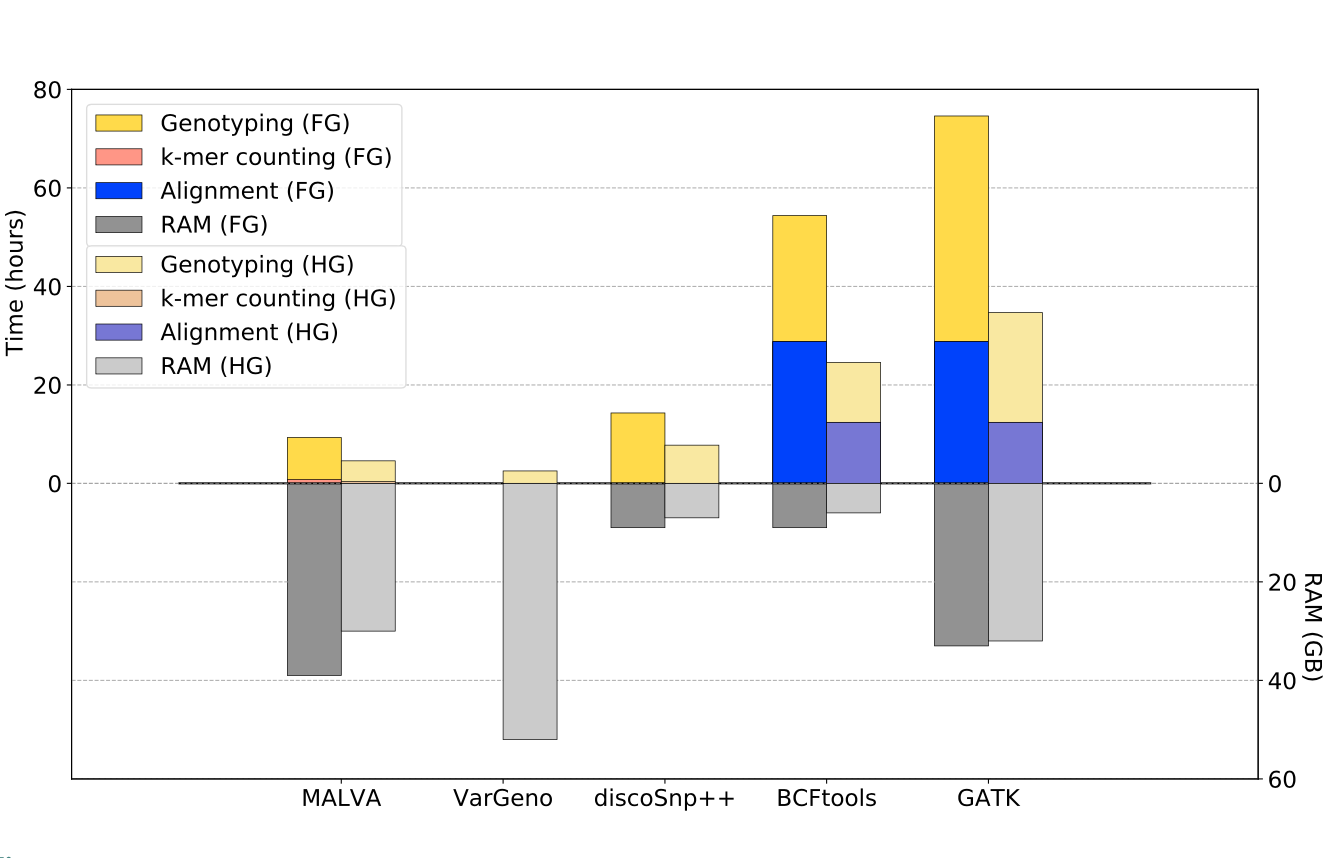
\includegraphics[scale=.39]{images/confronto1.png}
  \captionof{figure}{Tempo di esecuzione e utilizzo della memoria rispetto all'intero dataset \texttt{FullGenome}(FG, prima colonna) e a \texttt{HalfGenome}(HG, seconda colonna).}
  \label{fig:confronto1}
\end{minipage}%
\begin{minipage}{.5\textwidth}
  \centering
  \captionsetup{justification=centering}
%  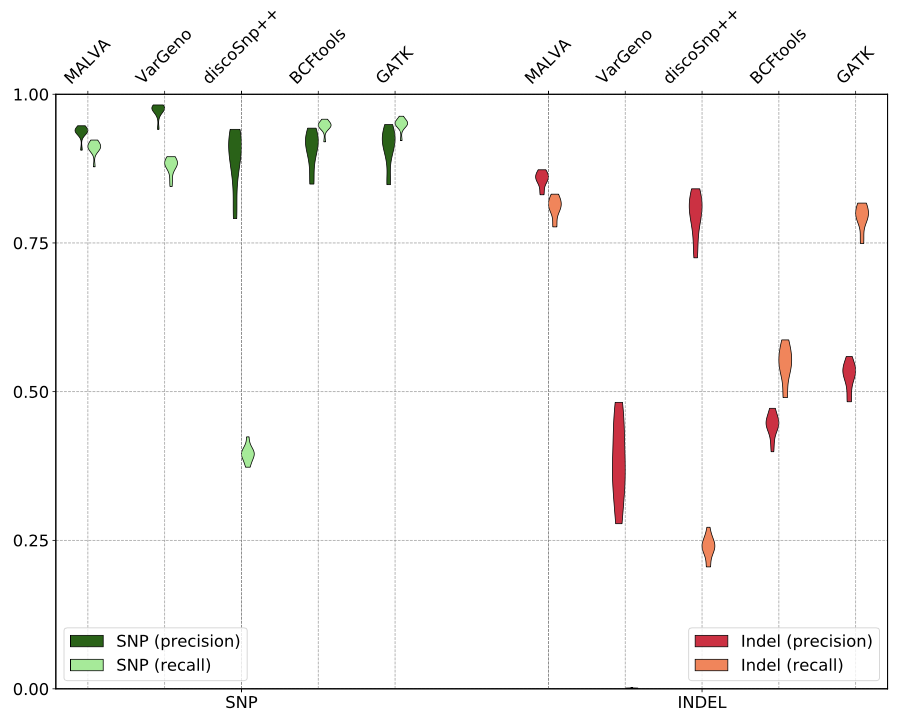
\includegraphics[scale=.50]{images/confronto2.png}
  \captionof{figure}{Rappresentazione qualitativa dell'accurancy rispetto a \texttt{HalfGenome} dataset.}
  \label{fig:confronto2}
\end{minipage}
\end{figure}

\noindent
Come previsto, MALVA, VarGeno e DiscoSnp\texttt{++} sono più veloci (rispettivamente 4.5, 2.5 e 7.5 ore) dei due approcci basati sull'allineamento testati (24.5 e 34.5 ore) che spendono molto tempo per l'allineamento.

Rispetto all'utilizzo di memoria, tra i tool \textit{mapping-free} DiscoSnp\texttt{++} si è rivelato l'approccio meno dispendioso, seguito da MALVA che aumenta il consumo di memoria di solo il 23\% per il dataset più grande. VarGeno invece richiede molta memoria, come già dichiarato nella relativa sezione: a causa della troppa memoria richiesta, non è stato possibile per gli autori completare il test sull'intero dataset, mentre per il dataset \texttt{HalfGenome} è stato utilizzato quasi il doppio di quella richiesta da MALVA nello stesso dataset.


La precisione e il richiamo di tutti gli strumenti sono relativamente elevate e comparabili: riportiamo delle considerazioni sul test con \texttt{HalfGenome} per poter confrontare anche VarGeno. VarGeno ottiene la miglior precisione sulle chiamate di SNP (97.5\%) rispetto a MALVA (93.8\%) e DiscoSnp\texttt{++} (89.5\%); questo perchè VarGeno preferisce non chiamare SNP in caso di incertezza mentre MALVA, per evitare la perdita di qualsiasi informazione potenzialmente interessante, preferisce rilevare qualsiasi potenziale allele alternato, a scapito di una leggera perdita di precisione. DiscoSnp\texttt{++} presenta il richiamo più basso (39.3\%) in confronto a MALVA (91.1\%) e VarGeno (88.1\%).


Sugli indel, MALVA ha ottenuto precisione e richiamo migliori rispetto agli altri tool. Come previsto, poiché VarGeno non è progettato per gestire gli indel, è stato in grado di genotipizzarne solo una bassa percentuale. DiscoSnp\texttt{++} invece, ha raggiunto un'alta precisione ma è stato in grado di chiamare solo meno di un quarto degli indel totali (24.2\%). I tool basati sull'allineamento hanno una bassa precisione rispetto agli indel, dovuta principalmente alle difficoltà di allineamento delle read che si sovrappongono agli indel. Analizzando inoltre la dimensione degli indel, MALVA si è rivelato l'unico strumento in grado di chiamare indel lunghi (oltre $\sim$40/50 basi), mentre gli altri strumenti sono limitati a indel brevi (che sono anche i più comuni): in ogni caso MALVA ha prestazioni migliori anche sugli indel corti, confermando di aver raggiunto l'obiettivo prefissato e di essere in grado di genotipizzare SNP multi-allelici e indel.\\

\noindent
Inoltre, \cite{bernardini2019malva} effettuano un confronto più approfondito tra MALVA e VarGeno, i due tool che hanno diverse componenti in comune (vedi Figura \ref{fig:confronto3}); gli indel non sono stati inclusi nell'analisi, poiché Vargeno non riesce ad individuarli.

\begin{figure}[h!]
	\centering
  	\captionsetup{justification=centering}
%  	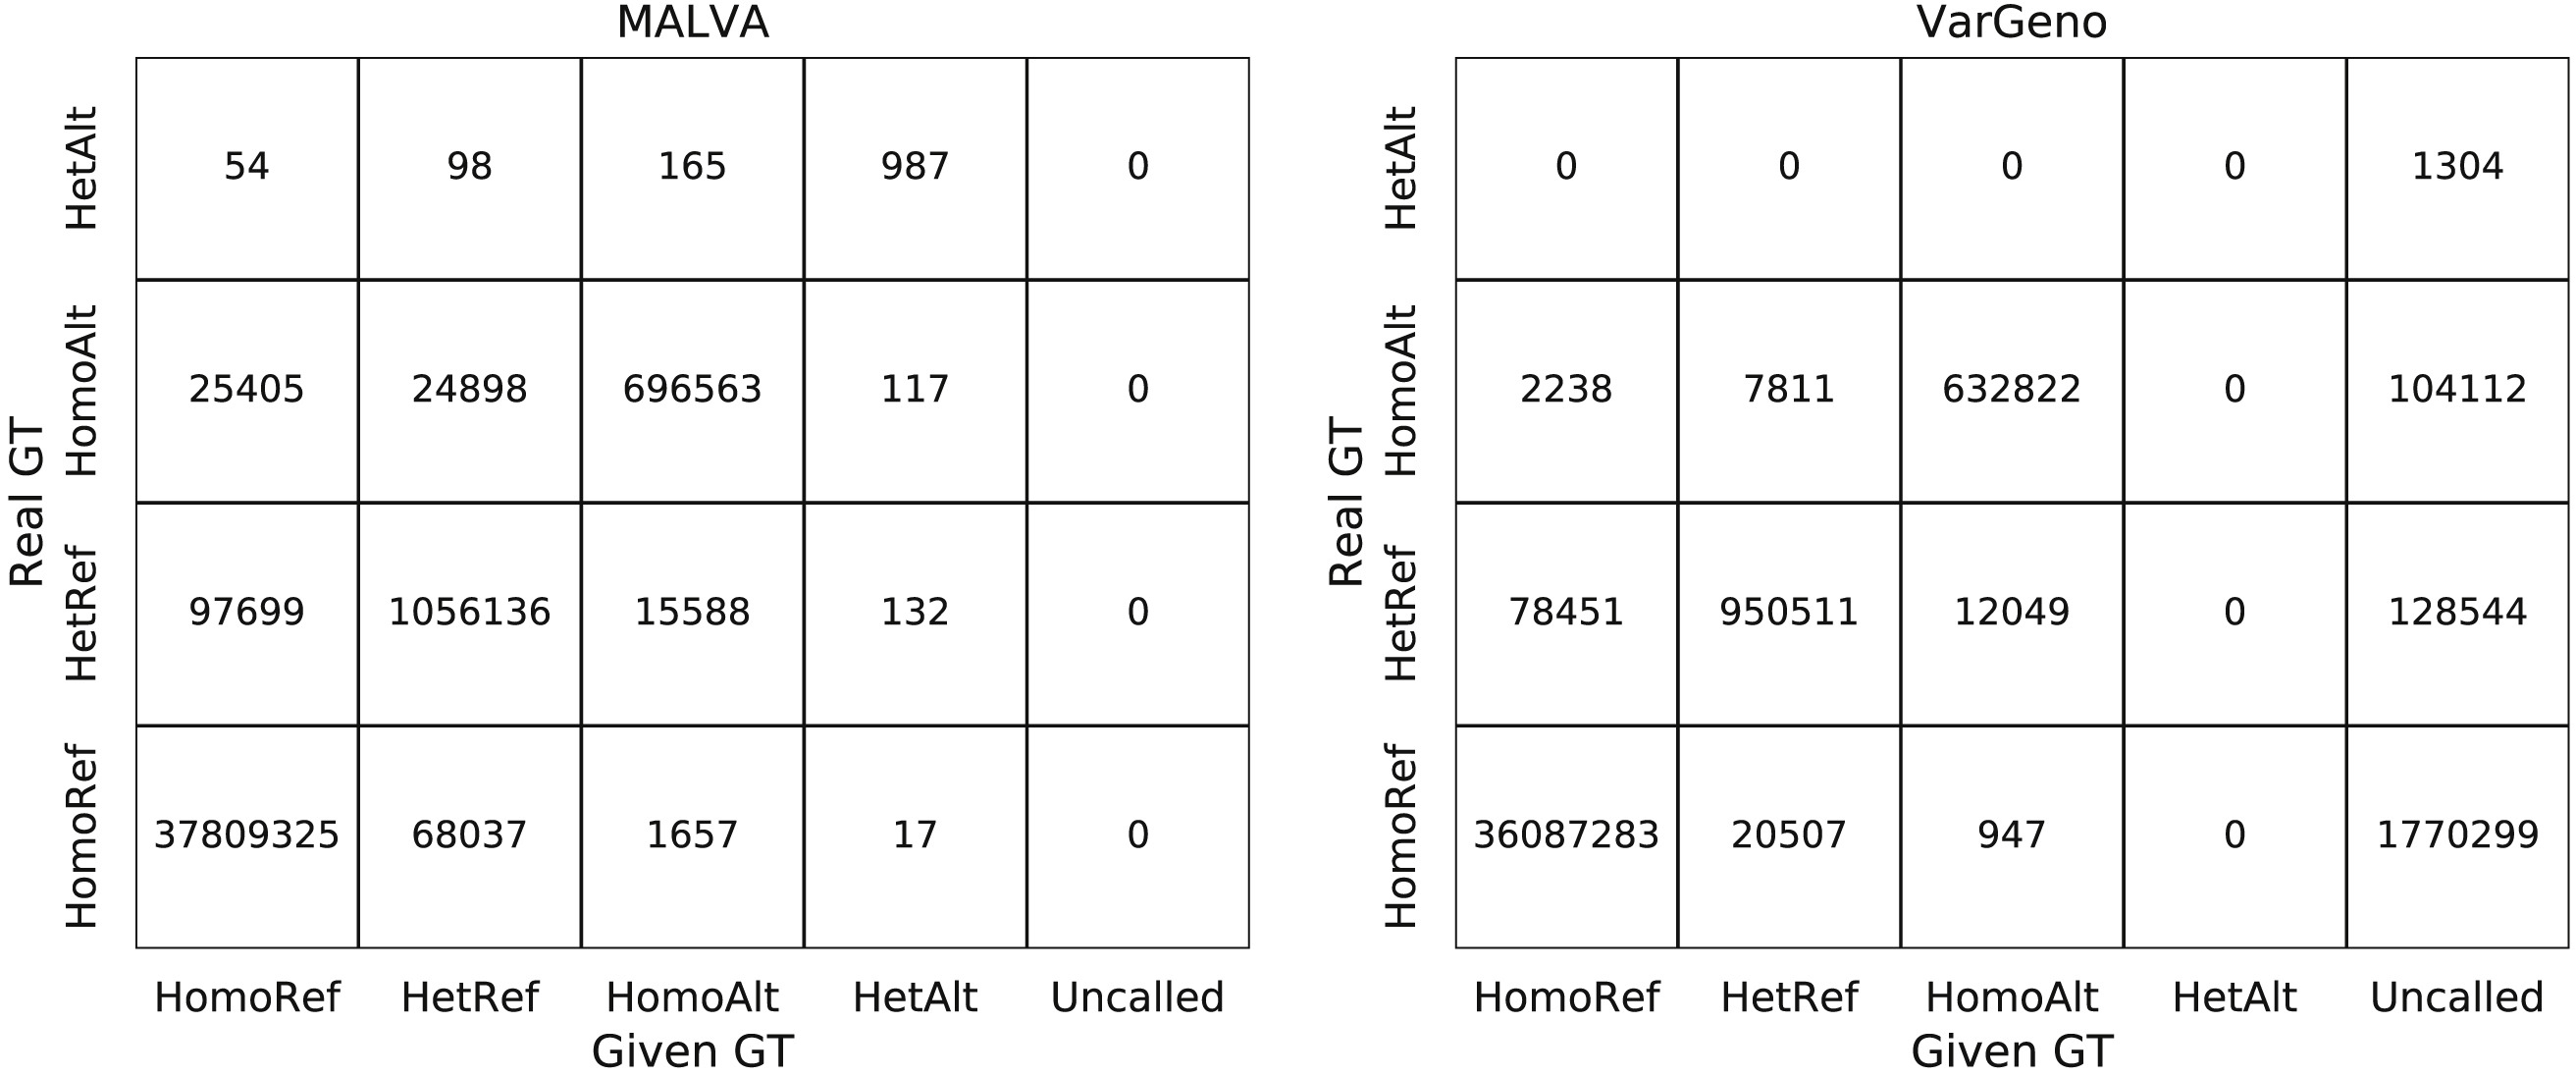
\includegraphics[scale=1.1]{images/confronto3.jpg}
  	\caption{Confronto (normalizzato per righe) tra genotipi reali (dataset 1000 Genome Project) e chiamati da MALVA e Vargeno.}
  	\label{fig:confronto3}
\end{figure}

\noindent
Per i due metodi viene riportato il numero di output di genotipi corretti, che viene confrontato con i reali genotipi, e nella figura, normalizzato per righe, raggruppandoli in riferimento omozigote (HomoRef), riferimento eterozigote (HetRef), alternato omozigote (HomoAlt) e alternati eterozigoti (HetAlt).

MALVA rileva tra il 5\% e il 10\% in più di  varianti corrette rispetto a VarGeno in tutte le classi, al costo di produrre chiamate più errate. Entrambi gli strumenti mostrano uno schema simile nelle chiamate errate: le varianti di riferimento omozigote erroneamente genotipizzate sono state predette come riferimento eterozigote e, viceversa, varianti di riferimento eterozigote erroneamente genotipizzate sono state principalmente predette come riferimento omozigote. Inoltre, le varianti alternate omozigoti non correttamente predette sono state per lo più chiamate come riferimento eterozigote da VarGeno, mentre MALVA ha distribuito uniformemente gli errori tra i genotipio riferimento omozigote e riferimento eterozigote. Infine, le varianti alternate eterozigoti non correttamente trovate sono state per lo più genotipizzate come varianti alternate omozigoti da MALVA: ciò significa che MALVA  è stato in grado di rilevare il fatto che l'allele non era l'allele di riferimento ma ha chiamato, in modo sbagliato, uno dei due alleli alternati del donatore. 




\end{document}
